\documentclass[12pt]{article}

\usepackage{sbc-template}

\usepackage{graphicx,url}
\usepackage{todonotes}
\usepackage{comment}
\usepackage[brazil]{babel}   
%\usepackage[latin1]{inputenc}  
\usepackage[utf8]{inputenc}  
\usepackage{float}
% UTF-8 encoding is recommended by ShareLaTex

     
\sloppy

\title{Testes Baseados em Propriedades: um Mapeamento Sistemático}

\author{André L. N. Gomes \inst{1}, Lucas G. S. Félix \inst{1}, Lucas Lagôa \inst{1}} 
\address{Departamento de Ciência da Computação -- Universidade Federal de São João del Rei (UFSJ)  \\ Sâo João del Rei -- MG -- Brasil \\ \email{andgomes95@gmail.com, lucasgsfelix@gmail.com, lucaslagoanogueira@hotmail.com}
}

\begin{document} 

\maketitle

\begin{abstract}
    With the grow of the software industry the task of make software with better quality has become a challenge. In this way, software testing became essencial to enterprises and researchers all over the world aiming to find failures in codes. One of the many categories that aim to make better software is property based testing. In this work we make a sistematic mapping objectiving give a overview in this topic. To make that we evaluate 346 articles in the literature, however, only 36 answer our search parameters. In our results we show the growth of this area, however, most of this academic prodution concetrates in a few authors.
\end{abstract}
     
\begin{resumo} 
  O crescimento da indústria de \textit{software} fez com houvesse uma busca por uma melhor qualidade dos mesmos. Assim o teste de \textit{software} almeja a qualidade do mesmo procurando a presença de falhas, sendo uma destas o teste de \textit{software} baseado em propriedade. Sendo assim, neste trabalho, realizamos uma revisão sistemática do tema, avaliando a literatura do mesmo em busca de responder questões levantadas. Na revisão sistemática feita foram encontrados inicialmente $348$ artigos dos quais $36$ atendiam aos critérios de busca. Em nossos resultados, vemos que há uma crescente em pesquisas sobre o tema, e que o mesmo se concentra-se em poucos autores.  
\end{resumo}

\section{Introdução}\label{sec:introducao}
	
	%% falo do aumento do número de acessos a informação e tecnlogia
	A expansão das tecnologias da informação e comunicação (TICs), proporcionou a população em geral um maior contato com dispositivos eletrônicos \footnote{https://www.telesemana.com/futurecom/pt/2014/10/08/mercado-nacional-de-tics-e-perspectivas-de-expansao/} como celulares, computadores e \textit{video games}. Estes dispositivos e outros são controlados pelos chamados \textit{softwares}, os quais proporcionam funcionalidades a estes limitadas de acordo com o \textit{hardware}. Estima-se que o valor despendido com \textit{software} no ano de 2019 será de 201 bilhões de dólares \footnote{https://www.itforum365.com.br/digital/transformacao-digital-esta-por-tras-da-expansao-do-mercado-de-software-veja-8-tendencias/}, justificando assim a utilização e a importância deste ramo.

	%% com expansão da utilização do software a necessidade de se testar softwares para que haja qualidade dos mesmos
	Com o crescimento do indústria do \textit{software} houve a necessidade de garantir a qualidade destes produtos ao usuário final, não apenas em grandes companhias, em programas de larga escala, mas também em \textit{softwares} mais simples. O custo causado por falhas em programas para dispositivos chegou em 1,1 trilhão de dólares em 2016 \footnote{http://www.base2.com.br/2017/03/20/falhas-em-software-provocaram-prejuizos-de-us-1-1-trilhao-em-2016/}, sendo que o montante consumido poderia ter sido evitado com teste de software.

	%% pensando nisso foram feitos diversos tipos de modelos para testes
	Pensando nestes fatos, pesquisadores e empresas desenvolvem e aplicam a cada ano diversos tipos de teste de software. Dentre eles temos, testes baseado em modelos, teste funcional, teste de integração, teste de regressão, entre outros, os quais podem ser aplicados em diferentes etapas do processo de desenvolvimento de software, contudo, possuem o mesmo objetivo final \cite{paiva2016aplicaccao}.

	%% dentre eles temos o property based testing, explico o que é o property based testing
	Uma das abordagens para assegurar a qualidade do \textit{software} presentes na literatura atualmente é o teste baseado em propriedades, o qual aproveita os princípios e expectativas em relação ao comportamento do código e utiliza estes para testar, ao invés de aplicar exemplos específicos \cite{fink1997property}. Em outras palavras, constrói-se os casos de teste de maneira que estes revelam a presença de falhas que não são reveladas pela execução direta do código. 

	%% Neste estudo, visamos dar uma visão geral sobre teste baseado em propriedades...
	Em virtude destes fatos, neste estudo, objetivamos dar uma visão geral sobre o teste baseado em propriedades fazendo uma investigação das pesquisas realizadas no tema, dado que de acordo com nossos conhecimentos existem poucos estudos que realizam tal. Para isso, utilizamos em nossa metodologia a técnica de revisão sistemática. A revisão sistemática é um método que tem como objetivo mensurar a extensão de um determinado tema na literatura por meio de uma busca de trabalhos da área \cite{petersen2008systematic}.

	O restante do artigo está dividido da seguinte forma. Na seção \ref{sec:trabalhos_relacioandos}, é apresentada a fundamentação teórica para o trabalho. Na seção \ref{sec:revisao_sistematica}, é apresentada a revisão sistemática deste trabalho, como protocolos e os passos para realizamos o processo. Em sequência, na seção \ref{sec:resultados} são apresentados os resultados de nossa pesquisa. Por fim, na seção \ref{sec:conclusao} é apresentada a conclusão de nossa trabalho e algumas propostas de trabalhos futuros.
\section{Fundamentação Teórica} \label{sec:trabalhos_relacioandos}
 Nesta seção, apresentaremos uma breve introdução sobre conceitos básicos de teste baseados em propriedade. Iniciaremos apontando a definição do que são propriedades. Após isto, indicaremos uma explicação do que são testes baseados em propriedades, comparando-os com testes unitários e apresentando bibliotecas que utilizam estes testes. %Por fim, indicaremos geradores, elemento importante para criação e automatização destes testes.
 
 \subsection{Propriedade}
 %\todo[inline]{DEFINIÇÃO DE PROPRIEDADE}
 O primeiro passo de teste baseado em propriedade é selecionar uma propriedade de um conjunto de propriedades genéricas, ou escolher alguma especifica do programa \cite{fink1997property}. As propriedades são regras gerais que descrevem o comportamento de um programa \cite{9781680506211}, em que devem ser aplicadas logicamente para todos os tipos de entradas e saídas, para cada trecho de código. Elas são operadas em alto nível, descrevendo genericamente o resultado esperado de uma operação. 
 %Ele também mostra a presença de defeitos, e não ausência, sendo este um princípio do Teste de Software \cite{delamaro2017introduccao}. 
 
 \subsection{Teste Baseado a Propriedades}
 %\todo[inline]{O QUE SÃO TESTE BASEADOS EM PROPRIEDADE}
 Testes baseados em propriedade tem como característica a especificação de diversas propriedades para garantir ao usuário que o programa atenda a propriedade declarada \cite{fink1997property}. Ele visa aproveitar os princípios e expectativas em relação ao comportamento do código e usá-los diretamente como um teste, ao invés de exemplos específicos. 
 %O primeiro passo é parar de pensar que o property-based testing é sobre testes. É sobre propriedades. \cite{9781680506211}
 %Quando esses testes são difundidos, ele tende a revelar mais falhas que não poderiam ser mostrado com exemplos.
 
 %\todo[inline]{diferenças de testes unitários}
 %procurar citação
 A qualidade dos testes de unidade tradicionais é puramente determinada pela habilidade do programador de pensar em todos os casos a serem cobertos, que é definida pela experiência, atenção a detalhes e conhecimento geral do programa. A expectativa do teste baseado em propriedade seria poder definir uma propriedade genérica que cobriria qualquer entrada passada para o programa de modo que cenários desconhecidos possam ser detectados. As ferramentas utilizadas nos testes baseados em propriedade proveem métodos para a geração de entradas aleatórias que exercitem as partes a serem testadas.
 
 %\todo[inline]{bibliotecas que utilizam}
 Dentre as bibliotecas que utilizam esta abordagem de teste, a mais conhecida é QuickCheck \footnote{Link do QuickCheck - http://hackage.haskell.org/package/QuickCheck}, para Haskell, que serviu de inspiração para diversos outros frameworks e bibliotecas. PropEr \footnote{Github do propEr - https://github.com/proper-testing/proper}, framework para Erlang; SwiftCheck \footnote{Github do SwiftCheck - https://github.com/typelift/SwiftCheck}, biblioteca para Swift; JSverify \footnote{Github do JSVerify - https://github.com/jsverify/jsverify}, para JavaScript; FsCheck \footnote{Github do FsCheck - https://github.com/fscheck/FsCheck}, ferramenta para .NET; junit-quickcheck\footnote{Github do junit-quickcheck - https://github.com/pholser/junit-quickcheck}, biblioteca que suporta escrita e execução de testes baseado em propriedade no JUnit do Java e Rantly \footnote{Github do Rantly - https://github.com/hayeah/rantly}, para Ruby são exemplos de ferramentas que sofreram influencia direta do QuickCheck.
 
 Além desta, existem outras aplicações como Steam\_data\footnote{Github do Steam\_Data - https://github.com/whatyouhide/stream\_data}, para geração de dados e teste baseado em propriedades para Elixir; GOlang Property TestER\footnote{Github do GopTer - https://github.com/leanovate/gopter}, biblioteca para GO e Hypothesis \footnote{Github do Hypothesis - https://github.com/HypothesisWorks/hypothesis}, é uma biblioteca avançada com implementações para Python, Ruby e Java.

 %\subsection{Geradores}
 
 %\todo[inline]{GERADORES}
\section{Revisão Sistemática} \label{sec:revisao_sistematica}


Nessa seção, apresentaremos uma revisão sistemática que foi desenvolvida no trabalho. 

\subsection{Protocolo}

Como citado anteriormente, a revisão sistemática tem como objetivo fornecer uma visão de uma certa área utilizando um processo rigoroso de coleta e avaliação \cite{petersen2008systematic}. Espera-se obter como resultado o entendimento das tendências da área sobre o tema pesquisado.  A definição do objetivo de pesquisa e das questões de pesquisa são apresentados a seguir. 

\begin{itemize}
    \item \textbf{Objetivo:} Identificar estudos que falem sobre o “property-based testing” e as aplicações até o momento.
    \item \textbf{Questões de pesquisa:} 
    \begin{enumerate}
        \item Quais são os estudos atuais sobre “property-based testing”?
        \item Quais são as ferramentas que suportam esse tipo de teste?
        \item Qual vertente do "property-based testing" está sendo mais utilizada?
        \item Em qual domínio está sendo mais aplicado?
        \item Quais são as vantagens e desvantagens da utilização do "property-based testing"?
        \item Quais são os maiores desafios encontrados pelos pesquisadores nessa área?
    \end{enumerate}
\end{itemize}

Partindo do objetivo e das questões de pesquisa foram definidas estratégias para realizar a busca e a seleção dos estudos.

\subsection{Busca e seleção de estudos}

A seleção dos estudos e a estratégia de busca foram definidos de acordo com os tópicos abaixo: 

\begin{itemize}
    \item \textbf{Critérios para seleção das fontes:} Os critérios empregados para a seleção das fontes utilizadas no trabalho seguiram as principais conferências, periódicos e simpósios em que são publicados estudos da área de Teste de Software.
    
    
    \item \textbf{Métodos de pesquisa:} Será utilizada uma busca automática na qual será criada uma \textit{string} de busca e a mesma será executada nas fontes selecionadas.
    
    
    \item \textbf{Palavras-chave:} \textit{test, software testing, property-based testing}
    
    
    \item \textbf{String de busca:} ("property-based testing" OR "property based testing" OR "property based test" OR "property-based test") 
    
    
    \item \textbf{Listagem das Fontes Selecionadas:} Springer\footnote{\url{http://www.springerlink.com/}}, IEEE\footnote{\url{http://ieeexplore.ieee.org}}, ACM\footnote{\url{http://portal.acm.org/dl.cfm}} e Elsevier-Science Direct\footnote{\url{http://www.sciencedirect.com/}}
\end{itemize}

\subsection{Critérios para seleção dos estudos}

Para selecionar os estudos, foram definidos alguns critérios de inclusão e exclusão que são apresentados a seguir:

\begin{itemize}
    \item \textbf{Critério 1:} artigos que tratem de teste de software
    
    
    
    \item \textbf{Critério 2:} artigos que tratem de \textit{Property-based}
    
    
    \item \textbf{Critério 3:} artigos completos em inglês ou português
    
    
    \item \textbf{Critério 4:} artigos com texto completo disponível na \textit{Web}
    
    
    \item \textbf{Critério 5:} artigos que possuem resumo
\end{itemize}


\subsection{Processo de seleção e extração dos estudos}

O processo para selecionar os estudos relevantes foi realizado na etapa de seleção.

\begin{itemize}
    \item \textbf{Processo de seleção:} Nesse processo, são identificados os estudos relevantes, de
acordo com a leitura do título, do resumo e das palavras-chave. Vale a pena ressaltar
que nessa etapa também são excluídos os trabalhos duplicados. A relevância dos artigos foi feita com base na
leitura de todo o artigo selecionado para verificar se este atende aos requisitos estabelecidos previamente.
 
\end{itemize}

A Tabela \ref{tab:resultados} apresenta os resultados da revisão sistemática em números de acordo com as bases selecionadas. 

\begin{table}[htbp]
\centering
\caption{Tabela Resultados Revisão Sistemática}
\label{tab:resultados}
\begin{tabular}{|c|c|c|c|}
\hline
\textbf{Fontes} & \textbf{Retornados} & \textbf{Seleção} \\ \hline
IEEE & 33 &  19  \\ \hline
Springer & 130 &  16  \\ \hline
ACM & 159 &  0  \\ \hline
Science-Direct & 26 & 1  \\ \hline
\textbf{TOTAL} & \textbf{348} & \textbf{36} \\ \hline
\end{tabular}
\end{table}

\section{Resultados} \label{sec:resultados}

	Nesta seção analisamos os resultados de nossa revisão sistemática. O propósito desta seção é dar uma visão geral de teste baseado em propriedades. Além disto, aproveitamos esta seção para responder as questões levantadas em nossa revisão sistemática.

	Para responder a primeira questão (\textit{Quais são os estudos atuais sobre "property-based testing "?}), são analisados os artigos que foram publicados entre 2017 e 2018. Dos trabalhos publicados em todo período de publicações $(2003-2018)$, cerca de $25,7\%$ foram publicados em 2017-2018, mostrando que este é um tema atual. Para uma melhor visualização do crescimento de publicações que envolvem testes baseados em propriedades, a Figura \ref{fig:crescimento}  mostra a evolução das publicações sobre do tema ao longo dos anos.

	\begin{figure}[!ht]
	  \centering
	  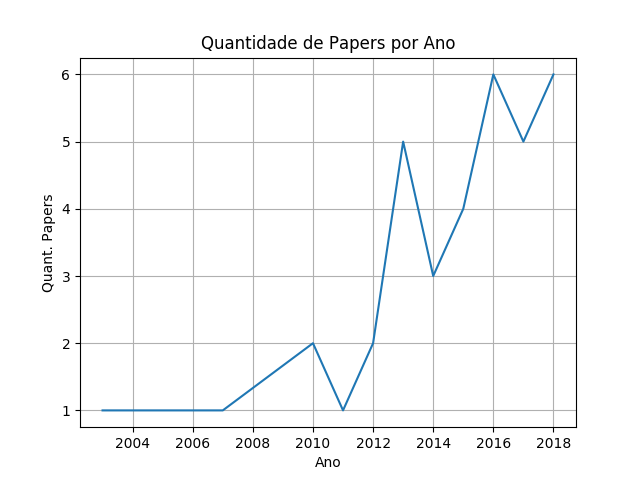
\includegraphics[scale=0.5]{Imagens/crescimento.png}
	  \caption{Crescimento do Teste Baseado em Propriedades ao longo dos anos}
      \label{fig:crescimento}
	\end{figure}

	Nos casos de estudo atuais do teste baseado em propriedades, há atualmente diferentes ramos de atuação dos artigos propostos. Grande parte dos artigos recentemente publicados utilizam o teste baseado em propriedades para aplicações,
	como \textit{web} \cite{peleg2018generating, martin2018property, chepurnoy2018checking, almendros2017web}  e \textit{block chain} \cite{aichernig2017property}. Enquanto alguns outros trabalhos \cite{loscher2018automating, hanus2016currycheck}, tem como objetivo o aperfeiçoamento deste tipo de teste. Em \cite{aichernig2017statistical} o teste baseado em propriedades é utilizado para simulação de modelos.


	%% qual vertente do property based testing está sendo mais usada -- considerando o tempo atual
	
	Sobre a segunda questão levantada (\textit{qual vertente do property based testing está sendo mais usada ?}), foi avaliado que grande maioria das aplicações de teste baseado em propriedades, considerando o tempo atual, são aplicações \textit{web}. Porém, além deste tipo de aplicações, existem abordagens em outros contextos como os já citados acima. Ao avaliarmos a quantidade de artigos publicados nos últimos anos (considerando período de $2017-2018$), cerca de $40\%$ são aplicações \textit{web}, o que nos auxiliou a chegar nesta conclusão. 

	%% quais são os pesquisadores mais influentes da área

	Para responder a quarta pergunta (\textit{quais são os pesquisadores mais influentes da área ?}) levantada na revisão sistemática, avaliamos os autores que mais publicam na área. Por meio da Figura \ref{fig:histograma} é perceptível que grande parte dos autores publicam apenas um artigo nesta área cerca de $72,2\%$. Enquanto outros autores, investem mais nessa área como por exemplo \textit{B. K. Aichernig e R. Schumi} os quais juntos possuem cerca de seis artigos na área, totalizando sozinhos $10\%$ dos artigos publicados no tema. Além desses, outros dois autores se destacam por ter dois artigos publicados na área, sendo eles: \textit{L. Fredlund et al} e \textit{K. Sagonas et al}.

	\begin{figure}[!ht]
	  \centering
	  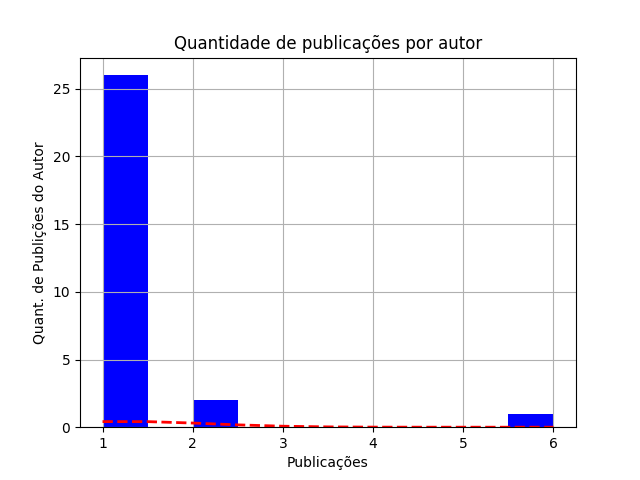
\includegraphics[scale=0.5]{Imagens/histograma.png}
	  \caption{Histograma que mostra a distribuição de artigos por autores}
      \label{fig:histograma}
	\end{figure}

	Avaliando quando estes artigos foram publicados, vemos que os autores \textit{B. K. Aichernig e R. Schumi} publicaram grande parte de seus artigos entre 2016-2018. Assim, concluímos que estes são os autores mais influentes nessa área em um período recente, dado o número de publicações e a abordagem das mesmas. Enquanto em um período menos recente, nos anos de 2014-2015 os autores que mais se destacam são \textit{L. Fredlund et al}.

	%% em qual domínimo está sendo aplicado

	Para avaliar os domínios em que a técnica de teste baseado em propriedades está sendo aplicada, foi realizada uma avaliação das palavras chaves presentes no artigo sendo estas sumarizadas por uma técnica de nuvem de palavras. Esta abordagem considera as palavras mais frequentes no texto para dar uma visão geral sobre as aplicações. Na Figura \ref{fig:cloud} é possível ver isto de maneira melhor.

	\begin{figure}[H]
	  \centering
	  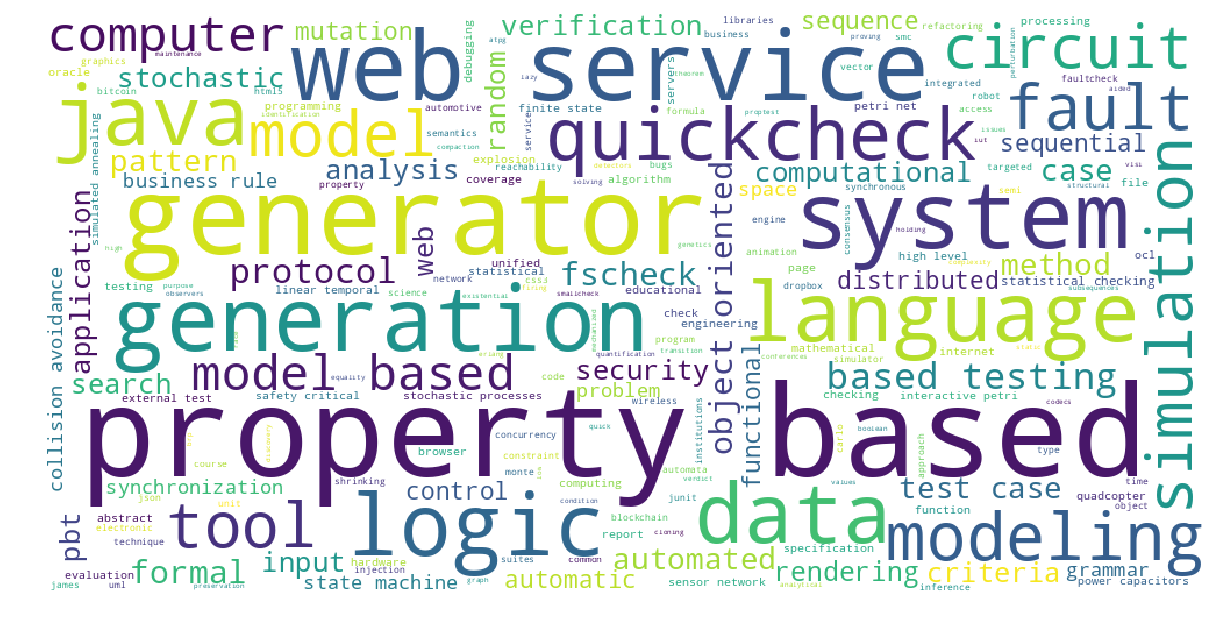
\includegraphics[scale=0.5]{Imagens/nuvem_palavras.png}
	  \caption{Nuvem de palavras}
      \label{fig:cloud}
	\end{figure}

	Por meio desta técnica de sumarização percebe-se que a abordagem é muito utilizada em linguagens \textit{web}, além de diversos paradigmas de programação como orientadas a objetos, funcionais e lógicas. Além destes, também é aplicada em domínios como segurança, \textit{block-chain} e mineração de dados (\textit{big data}), mostrando assim sua diversidade de aplicações e domínios, podendo esta ser aplicada em diversos contextos.
\section{Conclusão} \label{sec:conclusao}
    
    Neste trabalho é proposto um mapeamento sistemático com objetivo de dar uma visão geral ao teste baseado em propriedades. Para realizar tal tarefa, a revisão sistemática nos ajudou na coleta de diversos artigos presentes na literatura os quais tratam do teste baseado em propriedades. Após a leitura dos artigos, pode-se, assim, ter uma visão geral da dimensão desta área.
    
    Com base em nossos resultados, grande parte dos estudos publicados na área estão focados em testes para aplicações \textit{web}. Entretanto, em nossos estudos, foi percebido que há aplicações que fogem desta linha e mostram o potencial do teste baseado em propriedades o qual pode ser aplicado em diversos contextos como \textit{block-chain} e \textit{big data}.
    
    A novidade deste trabalho é que, nos limites de nosso conhecimento, este é o primeiro trabalho que realiza um mapeamento sistemático no tema de teste de \textit{software} baseado em propriedades.
    

\newpage
\bibliographystyle{sbc}
\bibliography{sbc-template}

\end{document}
